\documentclass{llncs}

\usepackage{graphicx}
\usepackage{amsmath,amssymb}
\usepackage{booktabs}
\usepackage{array}
\usepackage{url}
\usepackage[T1]{fontenc}
\usepackage{tikz}
\usetikzlibrary{positioning,arrows.meta}
\usepackage{pgfplots}
\pgfplotsset{compat=1.17}

% llncs.cls sets a narrow 12.2cm text block by design (matches Springer's
% printed page). Overriding it here with wider text and narrower side
% margins for on-screen / non-Springer-production reading.
\usepackage{geometry}
\geometry{a4paper, left=2.3cm, right=2.3cm, top=2.5cm, bottom=2.8cm}

\begin{document}

\title{MEV-Aware DeFi Liquidation: A Short Review}

\author{Priya Singh | Kashish Gupta | Vertika Singh | Avinash Kr. Ankur}
\institute{\email{priya.singh@jssaten.ac.in} |
\email{gptkashish973@gmail.com} |
\email{singhvertika119@gmail.com} |
\email{avinashhankur@gmail.com}\\
JSS Academy Of Technical Education, Noida}

\maketitle

\begin{abstract}
With strong applications in lending-protocol risk management, automated
market operations, and blockchain infrastructure design, liquidation in
decentralized finance (DeFi) is a fast-growing area of contemporary
blockchain research. A number of liquidation techniques sought to recover
undercollateralized debt using a fixed-incentive, priority-fee-driven
race among liquidators. However, Maximal Extractable Value (MEV)
research began to dominate the discussion once studies showed that this
race raises gas expenditure and can itself extract value from borrowers.
Auction and ordering mechanisms are used to structure competition and
then allocate the liquidation opportunity, so mechanism design in
liquidation is more crucial and challenging than it first appears. The
primary goal of this paper is to review the prominence of current
techniques, including both conventional priority-fee-based approaches
and MEV-aware, auction-based approaches.

\keywords{decentralized finance, DeFi, liquidation, maximal extractable value, MEV, auction mechanisms.}
\end{abstract}

\section{Introduction}

Decentralized lending protocols allow users to deposit collateral and
borrow against it without a centralized intermediary. Liquidation is the
process that keeps such protocols solvent: when a borrower's position
becomes undercollateralized, a third party, called a liquidator, repays
part or all of the outstanding debt and receives the collateral at a
discount in return. The goal of liquidation research is to determine how
this opportunity should be allocated among competing liquidators so that
debt is recovered quickly without imposing unnecessary cost on the
borrower or the protocol.

The problem is based on two fundamental ideas. The first is the
existence of the opportunity, that is, detecting that a position has
become undercollateralized. The second is allocation, that is, deciding
which liquidator gets to execute it and at what cost. By treating
liquidation as a transaction-ordering problem, researchers have connected
it to a wider phenomenon known as Maximal Extractable Value (MEV), the
profit that can be captured by controlling the order, inclusion, or
exclusion of transactions within a block~\cite{daian2019flash}. There is
continuous empirical research, together with mechanism-design proposals,
aimed at reducing the cost this competition imposes while keeping
liquidation fast enough to protect protocol solvency.

As illustrated in Fig.~\ref{fig:taxonomy}, current liquidation research
can be broadly classified into two categories: 1) conventional
priority-fee-based approaches and 2) MEV-aware, auction-based
approaches. Conventional approaches, such as fixed-spread liquidation and
raw priority-gas competition, rely on the existing transaction-ordering
market to decide the winner. MEV-aware approaches, by contrast,
restructure the competition itself, using auctions, batching, or
block-builder-aware scheduling to select a winner on efficiency grounds
rather than fee speed alone. Inspired by the growing research on these
two categories, this paper presents a short review of the methods
commonly used for MEV-aware liquidation.

\begin{figure}[h]
\centering
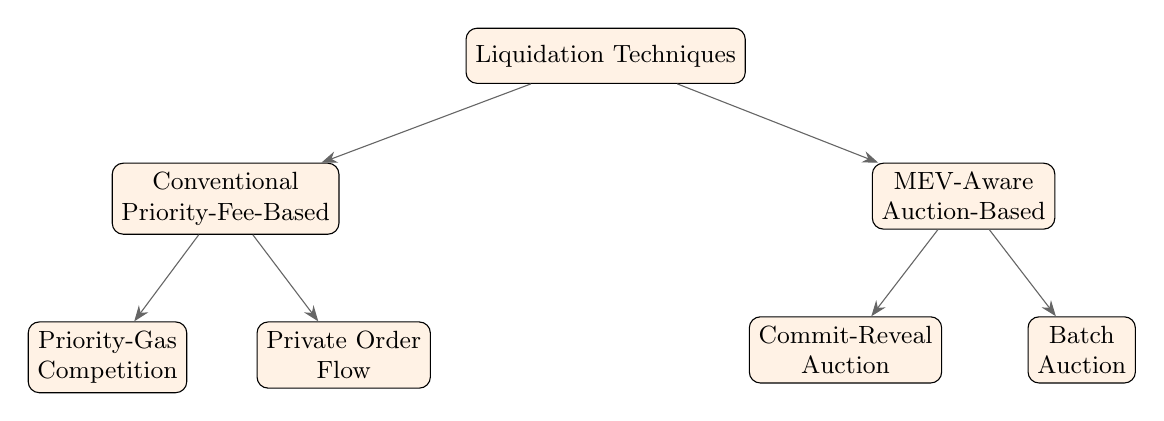
\begin{tikzpicture}[
  box/.style={draw, rounded corners, fill=orange!10, align=center, minimum height=0.7cm, font=\small},
  edge/.style={-{Stealth[length=2mm]}, draw, color=black!60}
]
\node[box] (root) {Liquidation Techniques};

\node[box, below left=1cm and 1.6cm of root] (conv) {Conventional\\Priority-Fee-Based};
\node[box, below right=1cm and 1.6cm of root] (mev) {MEV-Aware\\Auction-Based};

\node[box, below=1.1cm of conv, xshift=-1.5cm] (pgc) {Priority-Gas\\Competition};
\node[box, below=1.1cm of conv, xshift=1.5cm] (pof) {Private Order\\Flow};

\node[box, below=1.1cm of mev, xshift=-1.5cm] (cra) {Commit-Reveal\\Auction};
\node[box, below=1.1cm of mev, xshift=1.5cm] (ba) {Batch\\Auction};

\draw[edge] (root) -- (conv);
\draw[edge] (root) -- (mev);
\draw[edge] (conv) -- (pgc);
\draw[edge] (conv) -- (pof);
\draw[edge] (mev) -- (cra);
\draw[edge] (mev) -- (ba);
\end{tikzpicture}
\caption{Taxonomy of MEV-aware liquidation techniques.}
\label{fig:taxonomy}
\end{figure}

\section{Literature Review}
\label{sec:litreview}

This section places seven representative studies side by side and
compares them directly, rather than treating each as an isolated
citation. The studies were chosen to span the full liquidation
pipeline: detection of extractable value, measurement of its cost on
the public mempool, measurement of its cost inside private order flow,
and proposed fixes at the consensus and mechanism-design layers.
Table~\ref{tab:litreview} summarizes each study's focus, method, and
main limitation, and the discussion that follows groups the studies by
the layer of the pipeline they address and compares their findings
against one another.

\begin{table}[h]
\caption{Comparison of seven representative studies on MEV and DeFi liquidation.}
\label{tab:litreview}
\centering
\renewcommand{\arraystretch}{1.25}
\begin{tabular}{p{2.0cm}p{2.6cm}p{3.9cm}p{3.5cm}}
\toprule
\textbf{Study} & \textbf{Method} & \textbf{Key finding} & \textbf{Main limitation} \\
\midrule
Daian et al.~\cite{daian2019flash} (2019) &
Systems framework, case studies &
Coined and formalized MEV; unified front-running and reordering across DEXs and lending &
Largely conceptual; offers no liquidation-specific measurement \\
Qin et al.~\cite{qin2021empirical} (2021) &
Large-scale on-chain measurement &
Quantifies borrower loss from priority-gas competition across real liquidations &
Measures only the existing priority-fee regime, not alternative auctions \\
Torres et al.~\cite{torres2021frontrunner} (2021) &
Empirical detection over $\sim$11M blocks &
$\sim$200{,}000 front-running incidents found, liquidation races among them &
Detection heuristics may undercount activity hidden in private pools \\
Weintraub et al.~\cite{weintraub2022flashbot} (2022) &
Empirical measurement of a private pool &
Flashbots-connected miners held $>$99.9\% of hashing power in the period studied &
Single dominant provider studied; result is time- and provider-bound \\
Kelkar et al.~\cite{kelkar2020order} (2020) &
Protocol design, formal proofs &
Defines order-fairness guarantees at the consensus layer &
No liquidation-specific evaluation or latency cost estimate \\
Heimbach and Wattenhofer~\cite{heimbach2022sok} (2022) &
Systematization of knowledge (SoK) &
No surveyed countermeasure satisfies low latency, manipulation resistance, and decentralization at once &
Comparative and qualitative; introduces no new measurement \\
Wang et al.~\cite{wang2024private} (2024) &
Empirical and game-theoretic analysis &
Documents growing bidding concentration among a small number of block builders &
Forward-looking projection; concentration trend depends on how PBS evolves \\
\bottomrule
\end{tabular}
\end{table}

\textbf{Framework versus measurement.} Daian et al.~\cite{daian2019flash}
and Kelkar et al.~\cite{kelkar2020order} sit at the conceptual end of the
spectrum: the former supplies the vocabulary and systems framework that
every later measurement study relies on, while the latter proposes a
formal, consensus-layer fix. Neither paper measures liquidation activity
directly, which is exactly the gap that Qin et al.~\cite{qin2021empirical}
and Torres et al.~\cite{torres2021frontrunner} fill with large-scale
empirical studies. Comparing the two measurement studies directly,
Qin et al. focus on the economic outcome for the borrower within
lending protocols specifically, whereas Torres et al. measure
front-running incidents across DeFi more broadly and only report
liquidation races as one contributing category. The two are
complementary rather than conflicting: Qin et al. establish that the
loss is economically significant per event, and Torres et al. establish
that such events are not rare, at roughly 1.8\% of all blocks in their
sample (Fig.~\ref{fig:torres}).

\textbf{Public mempool versus private order flow.} Torres et
al.~\cite{torres2021frontrunner} and Weintraub et
al.~\cite{weintraub2022flashbot} measure the same underlying phenomenon,
MEV extraction, at two different points in the pipeline: the former in
the public mempool, the latter inside a single private-pool operator.
Read together, their results suggest that moving competition off the
public mempool does not remove concentration, it relocates it: Weintraub
et al. found over 99.9\% of hashing power connected to one private-pool
provider during the period studied (Fig.~\ref{fig:weintraub}), and
Wang et al.~\cite{wang2024private} later found a similar concentration
pattern one layer down, among block builders rather than miners. This
agreement across two independent studies, conducted on different
infrastructure and in different years, is stronger evidence for
structural concentration than either result would be alone.

\textbf{Design proposals versus their own trade-offs.} Kelkar et
al.~\cite{kelkar2020order} and Heimbach and
Wattenhofer~\cite{heimbach2022sok} both address the allocation side of
the problem rather than measuring it, but at different layers: Kelkar et
al. redesign the consensus protocol itself, while Heimbach and
Wattenhofer systematize application-layer and mechanism-level
countermeasures, commit-reveal and batch auctions among them. The SoK's
central finding, that no surveyed scheme achieves low latency,
manipulation resistance, and decentralization simultaneously, applies
directly to the four mechanisms compared in Table~\ref{tab:comparison}
and is visualized qualitatively in Fig.~\ref{fig:tradeoffs}: priority-gas
racing wins on latency but not manipulation resistance, while
commit-reveal and batch auctions trade latency away for the other two
properties.

\begin{figure}[h]
\centering
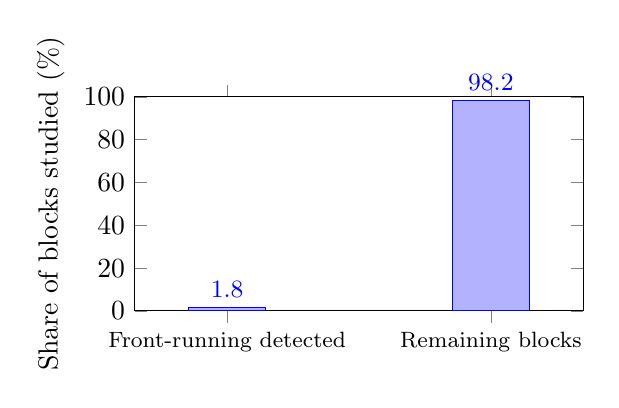
\begin{tikzpicture}
\begin{axis}[
    ybar,
    bar width=28pt,
    width=0.6\textwidth,
    height=4.3cm,
    symbolic x coords={Front-running detected,Remaining blocks},
    xtick=data,
    ymin=0, ymax=100,
    ylabel={Share of blocks studied (\%)},
    nodes near coords,
    every node near coord/.append style={font=\small},
    x tick label style={font=\footnotesize, align=center},
    enlarge x limits=0.35
]
\addplot coordinates {(Front-running detected,1.8) (Remaining blocks,98.2)};
\end{axis}
\end{tikzpicture}
\caption{Share of the $\sim$11 million Ethereum blocks studied by
Torres et al.~\cite{torres2021frontrunner} that contained at least one
detected front-running incident ($\sim$200{,}000 incidents in total).}
\label{fig:torres}
\end{figure}

\begin{figure}[h]
\centering
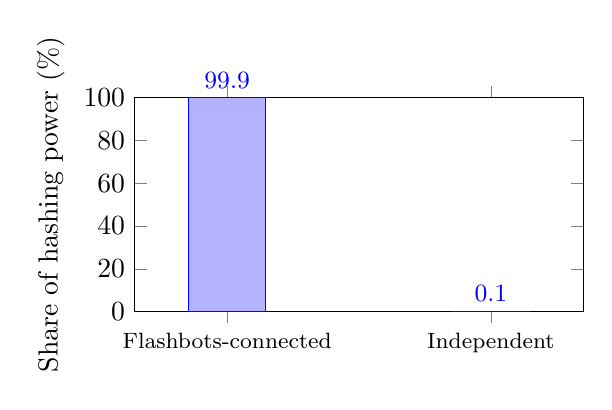
\begin{tikzpicture}
\begin{axis}[
    ybar,
    bar width=28pt,
    width=0.6\textwidth,
    height=4.3cm,
    symbolic x coords={Flashbots-connected,Independent},
    xtick=data,
    ymin=0, ymax=100,
    ylabel={Share of hashing power (\%)},
    nodes near coords,
    every node near coord/.append style={font=\small},
    x tick label style={font=\footnotesize, align=center},
    enlarge x limits=0.35
]
\addplot coordinates {(Flashbots-connected,99.9) (Independent,0.1)};
\end{axis}
\end{tikzpicture}
\caption{Share of Ethereum hashing power connected to Flashbots during
the period measured by Weintraub et al.~\cite{weintraub2022flashbot}.}
\label{fig:weintraub}
\end{figure}

\begin{figure}[h]
\centering
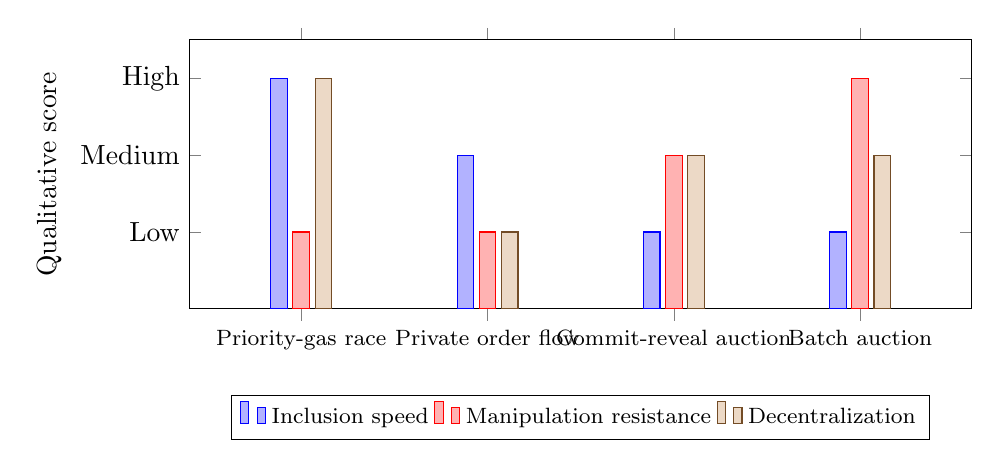
\begin{tikzpicture}
\begin{axis}[
    ybar,
    bar width=6pt,
    width=0.95\textwidth,
    height=5cm,
    symbolic x coords={Priority-gas race,Private order flow,Commit-reveal auction,Batch auction},
    xtick=data,
    ymin=0, ymax=3.5,
    ytick={1,2,3},
    yticklabels={Low,Medium,High},
    ylabel={Qualitative score},
    x tick label style={font=\footnotesize, align=center},
    legend style={font=\footnotesize, at={(0.5,-0.32)}, anchor=north, legend columns=-1},
    enlarge x limits=0.2
]
\addplot coordinates {(Priority-gas race,3)(Private order flow,2)(Commit-reveal auction,1)(Batch auction,1)};
\addplot coordinates {(Priority-gas race,1)(Private order flow,1)(Commit-reveal auction,2)(Batch auction,3)};
\addplot coordinates {(Priority-gas race,3)(Private order flow,1)(Commit-reveal auction,2)(Batch auction,2)};
\legend{Inclusion speed, Manipulation resistance, Decentralization}
\end{axis}
\end{tikzpicture}
\caption{Qualitative comparison of the four mechanisms in
Table~\ref{tab:comparison}, illustrating the trade-off Heimbach and
Wattenhofer~\cite{heimbach2022sok} identify across surveyed
countermeasures. Scores are illustrative summaries of the discussion in
this section, not measured data.}
\label{fig:tradeoffs}
\end{figure}

\section{Conventional Priority-Fee-Based Approaches}

According to Qin et al.~\cite{qin2021empirical}, liquidation outcomes can
be viewed at three levels: incentive design, execution cost, and
borrower impact. Incentive design fixes the discount a liquidator
receives; execution cost depends on the gas market at the moment of
liquidation; and borrower impact depends on how much collateral is lost
relative to the debt recovered. These three levels are used to model
most conventional liquidation mechanisms in use today. The foundational
work of Daian et al.~\cite{daian2019flash} applied a unified framework to
describe front-running and reordering risk across decentralized
exchanges and lending protocols alike. Competition for liquidation was
found to operate in two ways: 1) mempool-visible priority racing and 2)
private-channel submission. In the following subsections, these
techniques are covered in detail.

\subsection{Priority-Gas Competition}

A group of researchers~\cite{qin2021empirical} has studied how
liquidators bid gas prices against each other once a position becomes
eligible, a process that mirrors a first-price, continuous-time auction
over block space. The liquidator who is willing to pay the highest
priority fee usually wins inclusion, so the discount margin is
competed away toward the cost of the marginal gas bid. The empirical
study~\cite{qin2021empirical} found that this competition is real and
economically significant, but it also found that borrowers can lose
substantially more value than the protocol strictly needs to recover,
particularly during periods of high volatility. In a large-scale
measurement study, Torres, Camino, and State~\cite{torres2021frontrunner}
found close to 200{,}000 front-running incidents across roughly 11
million Ethereum blocks, showing that priority-gas competition is not a
theoretical concern but a persistent, high-volume feature of the
network, of which liquidation races form a significant share.

Front-running and transaction-reordering studies~\cite{daian2019flash}
summarized this competition as an instance of a broader
transaction-ordering market. Existing block-construction incentives were
used to explain why this market persists even as tooling around it
matures. Eskandari, Moosavi, and Clark~\cite{eskandari2019sok}
systematized front-running attack types on blockchains before the MEV
terminology was widely used; their taxonomy predates most of the
liquidation-specific literature but still underlies how later studies
classify priority-gas competition. According to this line of work, a
single gas bid cannot adequately capture a liquidator's true willingness
to pay, particularly when several liquidators are competing for the
same opportunity. Thus, later designs needed a richer signal than a
single priority fee to allocate the opportunity efficiently.

\subsection{Private Order Flow and Direct Submission}

An alternative to the public mempool race is to submit liquidation
transactions through private order flow, bypassing the public
transaction pool to avoid front-running by other searchers. Such
approaches shift competition away from the mempool and toward whichever
block builder or relay accepts the private transaction. Private
order-flow arrangements can reduce visible competition, but they also
concentrate market power in the hands of the builders who receive this
flow~\cite{wang2024private}. Weintraub et al.~\cite{weintraub2022flashbot}
measured this concentration directly for Flashbots, the most widely used
private-pool infrastructure, and found that Flashbots-connected miners
accounted for over 99.9\% of Ethereum's hashing power during the period
studied, even though Flashbots was designed to reduce, not concentrate,
the negative externalities of MEV competition. When too little of the
liquidation flow is public, the effective market for block space becomes
harder to observe and to reason about, while relying entirely on public
bidding can leave liquidators exposed to being outbid at the last
moment. Pai and Resnick~\cite{pai2023structural} extend the study of
this trade-off by examining how integrated builders gain structural
advantages over independent ones under this regime.

Priority-fee-based approaches produce results quickly and require no
protocol changes, but they are not necessarily efficient. Bidding
becomes wasteful as gas prices climb during volatile markets, since most
of the extra fee paid does not go toward recovering debt. It can be
costly and unpredictable for liquidators to participate under these
conditions, which makes the mechanism less attractive for smaller
searchers.

\section{MEV-Aware and Auction-Based Approaches}

Because of their ability to separate the question of who should win from
the question of how fast a transaction is included, auction mechanisms
are increasingly proposed for liquidation. An auction-based mechanism
collects bids or commitments from liquidators and selects a winner using
an explicit scoring rule rather than raw transaction-inclusion speed.
Heimbach and Wattenhofer~\cite{heimbach2022sok} systematized the wider
space of reordering-manipulation countermeasures in DeFi and found that,
across the schemes surveyed, none fully satisfied every property a
liquidation mechanism would want at once, namely low latency, resistance
to manipulation, and minimal impact on decentralization. This trade-off
motivates much of the auction-specific work reviewed below.
Kelkar et al.~\cite{kelkar2020order} developed order-fairness properties
for the underlying consensus layer to reduce a single party's ability to
manipulate transaction order for profit. It was followed by
mechanism-design work aimed at applying similar fairness guarantees
specifically to liquidation auctions. Deeper redesigns of the ordering
layer are prone to introducing new latency costs of their own.
Natale and Moser~\cite{natale2023cost} quantified the cost of
artificially delaying block proposal within a proposer-builder separation
(PBS) context, a cost that any batching or commit-reveal liquidation
auction must budget for. Ethereum.org's technical
documentation~\cite{ethereumorg} provides a continuously updated,
practitioner-facing description of how PBS, relays, and builders fit
together, and is a useful companion to the academic sources above for
readers unfamiliar with the current infrastructure, though as a living
document it should be read alongside the dated academic sources rather
than in place of them.

Werner et al.~\cite{werner2021sok} and Gogol et al.~\cite{gogol2024sok}
suggested a practical way of situating liquidation-specific mechanisms
within the broader systematization of DeFi risk. The studies
demonstrated that liquidation cannot be optimized in isolation from
other MEV-generating activities such as arbitrage, since the same
searchers and the same block-builder market participate in both.

Wang et al.~\cite{wang2024private} proposed a builder-bidding-dynamics
analysis for Ethereum's block-building market that could help predict
which liquidation-auction designs remain viable as private order flow
grows. The analysis, including bidding concentration among a small
number of builders, was used to explain the direction of the market. It
suggested caution for real-time auction designs that depend on
competitive, decentralized block building. When working on
auction-based liquidation, the Bank of Canada working
paper~\cite{bankofcanada2025} took a different approach compared to the
purely technical studies, evaluating liquidation mechanisms and price
impact from a financial-stability standpoint. The macro-level framework
decreased the reliance on purely searcher-level metrics. Instead, it
used protocol-level solvency outcomes that are less specific to any one
implementation.

Qin, Zhou, and Gervais~\cite{qin2022quantifying} highlighted the
limitations of narrow, single-metric measurement for extractable value
more broadly, in the context of contemporary MEV research. By
quantifying how much value remains extractable under different market
conditions, the study helped establish a benchmark against which
auction-based liquidation designs can be judged. It substantially
improved the ability to compare designs on a common empirical basis.
Table~\ref{tab:comparison} shows the advantages and disadvantages of
auction-based mechanisms relative to the priority-fee baseline.

\begin{table}[h]
\caption{Advantages and disadvantages of MEV-aware liquidation mechanisms.}
\label{tab:comparison}
\centering
\renewcommand{\arraystretch}{1.2}
\begin{tabular}{p{0.9cm}p{2.3cm}p{4.3cm}p{4.3cm}}
\toprule
\textbf{No.} & \textbf{Mechanism} & \textbf{Advantages} & \textbf{Disadvantages} \\
\midrule
1. & Priority-gas race & Simple, requires no protocol change & Wasteful bidding, unpredictable cost for liquidators \\
2. & Private order flow & Reduces visible front-running & Concentrates power in a few builders \\
3. & Commit-reveal auction & Scores bids on efficiency, not just speed & Reveal delay adds latency cost \\
4. & Batch auction & Aggregates competing bids into one clearing event & Batching window may allow price to move against the protocol \\
\bottomrule
\end{tabular}
\end{table}

\subsection{Challenges in MEV-Aware Mechanism Design}

Although the positive aspects of auction-based liquidation for reducing
execution cost have so far been demonstrated in isolated studies,
significant work is still needed to address the apparent problems. Real
searcher behavior has a significant influence on the accuracy of any
mechanism evaluated only in theory. Mechanisms are usually judged using
historical, priority-fee-era data, but there is a scarcity of data on
how strategic liquidators would actually bid under a redesigned auction.
Model mismatch and an unreliable efficiency estimate are caused by this
gap between theory and observed behavior. Latency is the main obstacle
when introducing a commit-reveal or batching step. Faster settlement
results from shorter reveal windows, while a more accurate, less
manipulable clearing price results from longer ones. A small share of
liquidation events is frequently responsible for most of the borrower
loss recorded in existing datasets. The remaining events, however, are
part of the low-volatility, low-competition regime. High importance is
given to these small, high-loss events for evaluation purposes, which
may also be taken into account when tuning a mechanism. Nevertheless, a
design tuned only toward the least common, highest-loss events risks
being biased away from the ordinary case that makes up most liquidation
volume.

\section{Conclusion}

In blockchain-based lending, protocol design favors mechanisms that
recover debt with more efficiency and less collateral loss than a raw
priority-fee race allows. We frequently overlook a number of additional
costs that are probably imposed on borrowers but may not be visible in
liquidator profit figures alone, because they are distributed across
many small events. MEV-aware liquidation is intended for both public
mempool and private order-flow environments. A liquidation event is
shaped by weaving together several forces: liquidator incentive, gas
market conditions, block-builder behavior, and borrower risk. To
evaluate mechanisms across these forces, isolate the effect of any one
design change, and ultimately recommend a mechanism, metrics like
execution cost, borrower loss, and inclusion latency are needed together
rather than one at a time.

Following the growth of proposer-builder separation and private order
flow, MEV research began to move beyond the priority-fee model that
defined early DeFi liquidation. By taking advantage of structured
bidding and explicit scoring rules to allocate the liquidation
opportunity, auction-based mechanisms were proposed to improve the
protocol's cost profile. Different auction-based liquidation proposals
are rich in reducing wasted gas expenditure, tightening the link between
bid and true willingness to pay, and, in principle, improving borrower
outcomes, whereas the priority-fee baseline was built on raw
transaction-inclusion speed alone. In liquidation-mechanism design,
commit-reveal and batch auctions are increasingly studied. However,
no single existing study jointly evaluates liquidator strategy,
execution cost, borrower loss, protocol recovery, and block-builder
interaction within one consistent experimental framework, which remains
an open problem for future work.

\begin{thebibliography}{15}

\bibitem{daian2019flash}
Daian, P., Goldfeder, S., Kell, T., Li, Y., Zhao, X., Bentov, I.,
Breidenbach, L., Juels, A.: Flash Boys 2.0: Frontrunning, Transaction
Reordering, and Consensus Instability in Decentralized Exchanges. arXiv
preprint arXiv:1904.05234 (2019).

\bibitem{qin2021empirical}
Qin, K., Zhou, L., Gamito, P., Jovanovic, P., Gervais, A.: An Empirical
Study of DeFi Liquidations: Incentives, Risks, and Instabilities. In:
Proc. ACM Internet Measurement Conference (IMC); 2021. p. 336--350.

\bibitem{qin2022quantifying}
Qin, K., Zhou, L., Gervais, A.: Quantifying Blockchain Extractable
Value: How Dark is the Forest? In: Proc. IEEE Symposium on Security and
Privacy (S\&P); 2022. p. 198--214.

\bibitem{kelkar2020order}
Kelkar, M., Zhang, F., Goldfeder, S., Juels, A.: Order-Fairness for
Byzantine Consensus. In: Proc. CRYPTO; 2020. IACR ePrint 2020/269.

\bibitem{werner2021sok}
Werner, S.M., Perez, D., Gudgeon, L., Klages-Mundt, A., Harz, D.,
Knottenbelt, W.J.: SoK: Decentralized Finance (DeFi). arXiv preprint
arXiv:2101.08778 (2021).

\bibitem{gogol2024sok}
Gogol, K., et al.: SoK: Decentralized Finance (DeFi): Fundamentals,
Taxonomy and Risks. arXiv preprint arXiv:2404.11281 (2024).

\bibitem{bankofcanada2025}
Bank of Canada: Liquidation Mechanisms and Price Impacts in DeFi. Staff
Working Paper 2025-12 (2025).

\bibitem{pai2023structural}
Pai, M., Resnick, M.: Structural Advantages for Integrated Builders in
MEV-Boost. arXiv preprint arXiv:2311.09083 (2023).

\bibitem{wang2024private}
Wang, Y., et al.: Private Order Flows and Builder Bidding Dynamics: The
Road to Monopoly in Ethereum's Block Building Market. arXiv preprint
arXiv:2410.12352 (2024).

\bibitem{natale2023cost}
Natale, M., Moser, S.: The Cost of Artificial Latency in the PBS
Context. arXiv preprint arXiv:2312.09654 (2023).

\bibitem{eskandari2019sok}
Eskandari, S., Moosavi, S., Clark, J.: SoK: Transparent Dishonesty:
Front-Running Attacks on Blockchain. arXiv preprint arXiv:1902.05164
(2019).

\bibitem{ethereumorg}
Ethereum.org: Maximal Extractable Value (MEV). \url{https://ethereum.org/developers/docs/mev}, accessed 2026.

\bibitem{torres2021frontrunner}
Torres, C.F., Camino, R., State, R.: Frontrunner Jones and the Raiders
of the Dark Forest: An Empirical Study of Frontrunning on the Ethereum
Blockchain. In: Proc. 30th USENIX Security Symposium; 2021. p.
1343--1359.

\bibitem{weintraub2022flashbot}
Weintraub, B., Torres, C.F., Nita-Rotaru, C., State, R.: A Flash(bot) in
the Pan: Measuring Maximal Extractable Value in Private Pools. In: Proc.
22nd ACM Internet Measurement Conference (IMC); 2022. p. 458--471.

\bibitem{heimbach2022sok}
Heimbach, L., Wattenhofer, R.: SoK: Preventing Transaction Reordering
Manipulations in Decentralized Finance. In: Proc. 4th ACM Conference on
Advances in Financial Technologies (AFT); 2022. p. 47--60.

\end{thebibliography}

\end{document}